\documentclass[11pt]{article}
\usepackage[margin=1in]{geometry}
\usepackage{amsmath,amssymb,amsthm,graphicx,caption}
\usepackage[T1]{fontenc}
\usepackage{lmodern,microtype}
\usepackage{needspace}
\usepackage[hidelinks]{hyperref}
\raggedbottom
\clubpenalty=10000
\widowpenalty=10000
\displaywidowpenalty=10000
\captionsetup{font=small,hypcap=false}
\newtheorem{proposition}{Proposition}
\setlength{\parskip}{3pt}
\makeatletter
\renewcommand\paragraph{\@startsection{paragraph}{4}{\z@}
 {1.5ex plus .5ex minus .2ex}{-1em}{\normalfont\normalsize\bfseries}}
\makeatother
\title{How Closely Can a Discrete Space\\Imitate Continuum Waves?}
\author{J. R. Landers}
\date{November 13, 2026}
\begin{document}
\maketitle
\begin{abstract}
If distinct positions are separated by a minimum distance, must waves reveal it? Earlier work followed this premise from elementary geometry to a lattice model in which high-frequency waves travel more slowly, suggesting astronomical photon timing as a possible test. This note asks how much of that signal belongs to the spacing and how much to the chosen interactions. On the same lattice, positive pair interactions impose a definite phase-speed error. Allowing signed interactions while keeping the total energy nonnegative changes the answer: standard centered finite-difference rules can make both phase and group speeds arbitrarily close to their continuum values on any fixed band below the lattice cutoff, without exceeding the long-wavelength group speed. Finite interaction range still prevents exact agreement, and the cutoff retains a distinct signature. The result identifies a question that comes before detector sensitivity: which dynamics does a proposed minimum-distance model actually require? These are mathematical model comparisons, not evidence that physical space is discrete.
\end{abstract}

\section{Must a minimum distance leave a wave signature?}
Suppose there is a smallest separation $k$ between distinct positions. What would change, and how could we notice? The original minimum-distance exposition \cite{minimum} begins with consequences that need no equation of motion: some Euclidean triangles become impossible, repeated bisection must stop, and a continuous point trajectory cannot move through a uniformly discrete space. These are consequences of the geometry itself.

To detect that geometry, we need a physical process that carries its effects into a measurement. The original lattice-wave model makes short waves travel more slowly than long ones. If photons inherit this law, a small speed difference could accumulate over an astronomical journey into an arrival-time difference. The photon-timing companion \cite{timing} examined published observations; its limits leave the nearest-neighbor Planck-spacing prediction far below current sensitivity.

Before seeking greater sensitivity, however, we should ask: \emph{is the slowdown unavoidable, or did the interaction law put it there?} We keep the spacing fixed and change only the interactions. First we show that positive pair couplings cannot remove the discrepancy. We then construct stable signed couplings that make it as small as desired below the lattice cutoff, and ask what differences survive.

\subsection{Keeping the geometry fixed}
Take positions $x_n=nk$, indexed by the integer $n$. The real amplitude $u_n(t)$ lives at site $n$; it can vary continuously even though the sites are discrete. We retain the equation
\begin{equation}
 \ddot u_n=\frac{c^2}{k^2}\sum_{r=1}^R a_r
 (u_{n+r}-2u_n+u_{n-r}),\qquad \sum_{r=1}^R a_r r^2=1.
\end{equation}
The range $R$ counts how many lattice steps an interaction can span. The dimensionless coefficients $a_r=g_r k^2/c^2$ may have either sign. Their normalization fixes the same long-wavelength speed $c$ for every model.

A plane wave has wave number $q$ and angular frequency $\omega$. Write $x=qk$ for its dimensionless wave number, and collect the effect of all interactions in the function
\begin{equation}\label{symbol}
 D(x)=4\sum_{r=1}^R a_r\sin^2(rx/2),\qquad
 \omega(q)=\frac{c}{k}\sqrt{D(qk)}.
\end{equation}
An ideal continuum wave would have $D(x)=x^2$ and hence $\omega=cq$ for $q>0$. The lattice has independent wave numbers only in $|x|\leq\pi$, its \emph{Brillouin zone}: samples at the sites cannot distinguish wave numbers differing by $2\pi/k$. The edge $x=\pi$ corresponds to wavelength $2k$.

We compare two speeds. The phase speed $v_p=\omega/q$ describes the motion of a wave crest; the group speed $v_g=d\omega/dq$ describes the motion of a narrow wave packet and connects to the earlier arrival-time calculation. In this notation,
\begin{equation}
 \frac{v_p}{c}=\frac{\sqrt{D(x)}}{x},\qquad
 \frac{v_g}{c}=\frac{D'(x)}{2\sqrt{D(x)}}\quad (0<x<\pi)
\end{equation}
and both ratios equal one in the continuum model. Their limits at zero are one by normalization. A comparison band $0\leq x\leq X$ specifies the range of wavelengths an observation or calculation probes; $X<\pi$ means that it stops short of the lattice cutoff.

\subsection{What counts as an admissible interaction?}
Positive pair couplings give a familiar restoring force between each pair of sites. We will also allow negative pair coefficients, provided the complete system remains stable. The relevant condition is $D(x)\geq0$ for every lattice wave number: squared frequencies, and equivalently the total quadratic potential energy, must be nonnegative. A negative contribution from one pair need not make the sum negative.

Stability here means no exponential growth of normal modes; the acoustic zero mode has its usual uniform translation and velocity solutions. This is the requirement we test, rather than a claim that every such interaction is physically realized. Neither spectral stability nor a group-speed bound asserts a strict causal front or a relativistic theory.

\section{A sharp limitation for positive interactions}
The simplest attempt to hide the spacing is to add interactions with more distant sites. Can that bring the waves closer to continuum propagation? If every pair coupling is positive, the answer is no: nearest neighbors already give the largest phase speed at each wave number.

To see this, suppose $a_r\geq0$ and write $w_r=a_r r^2$, so that $\sum_r w_r=1$. The elementary inequality $|\sin(rt)|\leq r|\sin t|$ gives
\begin{equation}\label{positive}
 D(x)=4\sum_r w_r\left(\frac{\sin(rx/2)}{r}\right)^2
 \leq4\sin^2(x/2)\leq x^2.
\end{equation}
The first upper bound is precisely the nearest-neighbor dispersion relation; the second is the continuum one. Thus the nearest-neighbor rule $a_1=1$ maximizes the phase speed at every $x$. Longer positive interactions cannot improve its phase accuracy anywhere in $0<x\leq\pi$. In particular, for a fixed comparison band $0\leq x\leq X\leq\pi$,
\begin{equation}
 \inf_{a_r\geq0}\ \sup_{0\leq x\leq X}
 \left|\frac{v_p(x)}c-1\right|
 =1-\frac{\sin(X/2)}{X/2}.
\end{equation}
Even the best positive rule has a nonzero worst phase-speed error on a nontrivial band. Nearest neighbors attain the infimum, regardless of the allowed range. This argument does not order group-speed errors pointwise.

For the connection to timing, expand at small $x$. This recovers the earlier leading coefficient:
\begin{equation}
 D(x)=x^2-\frac{\mu_4x^4}{12}+O(x^6),\qquad
 \mu_4=\sum_r a_r r^4\geq1,
 \qquad \frac{v_g}{c}=1-\frac{\mu_4x^2}{8}+O(x^4).
\end{equation}
For this positive class, $\Lambda^2=k^2\mu_4\geq k^2$. The quadratic slowdown therefore has a lower coefficient at fixed spacing, which is what made the earlier photon test possible. Positivity does real work in this conclusion. Once signed couplings are admitted, $\mu_4$ can vanish or become negative and must not automatically be interpreted as the square of a real effective length. The next question is whether that freedom can remove the slowdown without making the waves unstable.

\section{A stable family with arbitrarily small band error}
\subsection{Canceling an error without shrinking the spacing}
A concrete example shows the possibility. The range-two rule $(a_1,a_2)=(4/3,-1/12)$ still has $a_1+4a_2=1$, so its long-wavelength speed is $c$. But $a_1+16a_2=0$: the coefficient $\mu_4$ vanishes, removing the quadratic group-speed correction. The spacing has stayed exactly the same.

This is the first member beyond nearest neighbors of a familiar construction from numerical differentiation \cite{nist,fornberg}. For each range $R$, take the centered coefficients
\begin{equation}\label{centered}
 a_r^{(R)}=\frac{2(-1)^{r+1}(R!)^2}{r^2(R-r)!(R+r)!},\qquad 1\leq r\leq R.
\end{equation}
For example, $R=1$ gives $(1)$, $R=2$ gives $(4/3,-1/12)$, and $R=3$ gives $(3/2,-3/20,1/90)$. In numerical analysis these weights approximate a continuum derivative from samples. Here they define the actual interactions of a candidate lattice model. The formulas are standard; the question is what they imply for waves if the lattice is taken literally.

\Needspace{11\baselineskip}
\subsection{Why the signed rules are stable}
Canceling a coefficient would be of little use if the resulting waves grew exponentially. An equivalent form makes stability transparent. Set $y=\sin^2(x/2)$, which lies between zero and one throughout the zone, and write
\begin{equation}\label{poly}
 D_R(x)=P_R(y),\qquad
 P_R(y)=\sum_{m=1}^R b_m y^m,\qquad
 b_m=\frac{2\,4^m}{m^2\binom{2m}{m}}>0.
\end{equation}
The infinite series is $4\arcsin^2\sqrt y=x^2$ for $0\leq x\leq\pi$. Thus the continuum target can be built by adding positive powers of $y$, and the range-$R$ rule keeps its first $R$ terms. Each truncation is a cosine polynomial of range $R$, and expansion gives Eq.~\eqref{centered}. Positivity of every $b_m$ implies $D_R(x)>0$ for $0<|x|\leq\pi$, proving stability at every wave number.

There is also a direct energy certificate. With the forward difference $(\Delta u)_n=u_{n+1}-u_n$, the total energy can be written
\begin{equation}
 H=\frac12\|\dot u\|^2+
 \frac{c^2}{2k^2}\sum_{m=1}^R\frac{b_m}{4^m}\|\Delta^m u\|^2\geq0.
\end{equation}
This applies on a periodic lattice or for sufficiently decaying data. Each term is a positive coefficient times a squared difference, so the total energy cannot be negative. The signed pair description and the positive total-energy description are two ways of writing the same dynamics. A chain made exclusively of positive pair springs would instead return us to Eq.~\eqref{positive}.

\subsection{How much of the signal can disappear?}
The range-two example extends to cancellation of the even moments through order $2R$ beyond the normalization:
\begin{equation}
 D_R(x)=x^2-C_Rx^{2R+2}+O(x^{2R+4}),\qquad
 C_R=\frac{2(R!)^2}{(2R+2)!}>0,
\end{equation}
and hence
\begin{equation}\label{grouporder}
 \frac{v_g}{c}=1-\frac{2R+1}{2}C_Rx^{2R}+O(x^{2R+2}).
\end{equation}
The first slowdown is quadratic at $R=1$, quartic at $R=2$, and of order $x^{2R}$ in general. Every increase in range pushes the first correction to a higher power of wave number. A universal nonzero quadratic delay therefore does not follow from stability and minimum spacing alone.

This also controls a whole band, rather than just a leading term near zero. For every fixed $X<\pi$, the series for $P_R$ and its derivative converge uniformly on $0\leq y\leq\sin^2(X/2)<1$. Factoring out $4y$ handles the acoustic limit without dividing by zero. It follows that both $v_p/c$ and $v_g/c$ converge uniformly to one on $[0,X]$ as $R$ grows, while the spacing $k$ remains fixed. Given a band below the cutoff and any positive error tolerance, some finite range meets that tolerance. The family also satisfies $0\leq v_g\leq c$ throughout the positive half-zone; a proof is given in Appendix~\ref{app:speed}. Making the lattice difficult to distinguish this way does not require a group-speed overshoot.

\section{How close do the waves get?}
How much improvement do modest ranges deliver? The script \texttt{study.py} compares centered rules at ranges $1,2,3,4,6,8,12,16$ on bands ending at $\pi/4$, $\pi/2$, and $3\pi/4$.

Canceling successive low-wave-number terms need not minimize error on a particular band. To explore that tradeoff, the script also optimizes a stability-certified subclass,
\begin{equation}
 P(y)=4y+\sum_{m=2}^R b_m y^m,\qquad b_m\geq0,
\end{equation}
minimizing $\sup_{[0,X]}|D(x)/x^2-1|$, the largest error in the squared phase-speed ratio. The constraints are linear in the coefficients; their nonnegativity guarantees stability over the full zone. The sampled linear program is refined at candidate extrema. This searches one stable subclass and does not prove an exact continuous minimax optimum.

For $X=\pi/2$, corresponding to wavelengths at least $4k$, the maximum speed errors are:
\begin{center}
\small
\begin{tabular}{llrr}
\hline
Family & Range $R$ & Max. phase error & Max. group error \\ \hline
Centered & 1 & $9.97\times10^{-2}$ & $2.93\times10^{-1}$ \\
Centered & 2 & $2.75\times10^{-2}$ & $1.27\times10^{-1}$ \\
Centered & 4 & $3.37\times10^{-3}$ & $2.66\times10^{-2}$ \\
Centered & 6 & $5.27\times10^{-4}$ & $5.87\times10^{-3}$ \\
Band-optimized & 2 & $6.00\times10^{-3}$ & $7.91\times10^{-2}$ \\
Band-optimized & 4 & $6.68\times10^{-5}$ & $3.59\times10^{-3}$ \\
Band-optimized & 6 & $2.12\times10^{-6}$ & $2.21\times10^{-4}$ \\
\hline
\end{tabular}

\end{center}
At range four, optimization reduces the phase error from approximately $0.337\%$ to $0.00668\%$, and the group error from $2.66\%$ to $0.359\%$. The objective uses the squared phase-speed ratio; the table reports phase-speed and group-speed errors separately. These are dense-grid estimates of model errors, not experimental uncertainties.

Figures~\ref{fig:dispersion} and~\ref{fig:convergence} show how the centered family improves as range grows, and where the lattice cutoff still intervenes.

That improvement has a tradeoff. Some optimized rules restore a lower-order dispersion term and permit group speeds above $c$: the range-four maximum is about $1.00073c$ over the full zone. Energy stability does not forbid this. A group-speed cap, already met by the centered family, would require another optimization constraint. Thus ``closest to the continuum'' needs a specified band, error measure, and physical restrictions.

\begin{center}
\begin{minipage}{\linewidth}
\centering
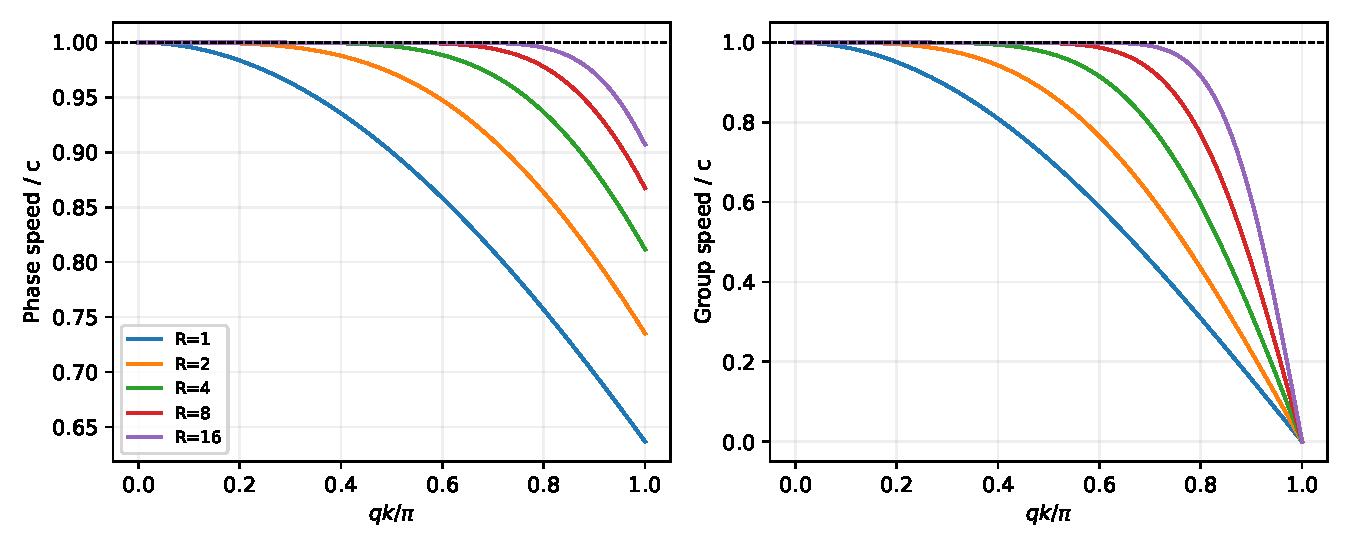
\includegraphics[width=.92\linewidth]{figures/dispersion.pdf}
\captionof{figure}{Centered rules approach continuum propagation over larger portions of the lattice spectrum as range increases. Every finite-range curve still has zero group speed at the zone edge.}\label{fig:dispersion}
\end{minipage}
\end{center}
\begin{center}
\begin{minipage}{\linewidth}
\centering
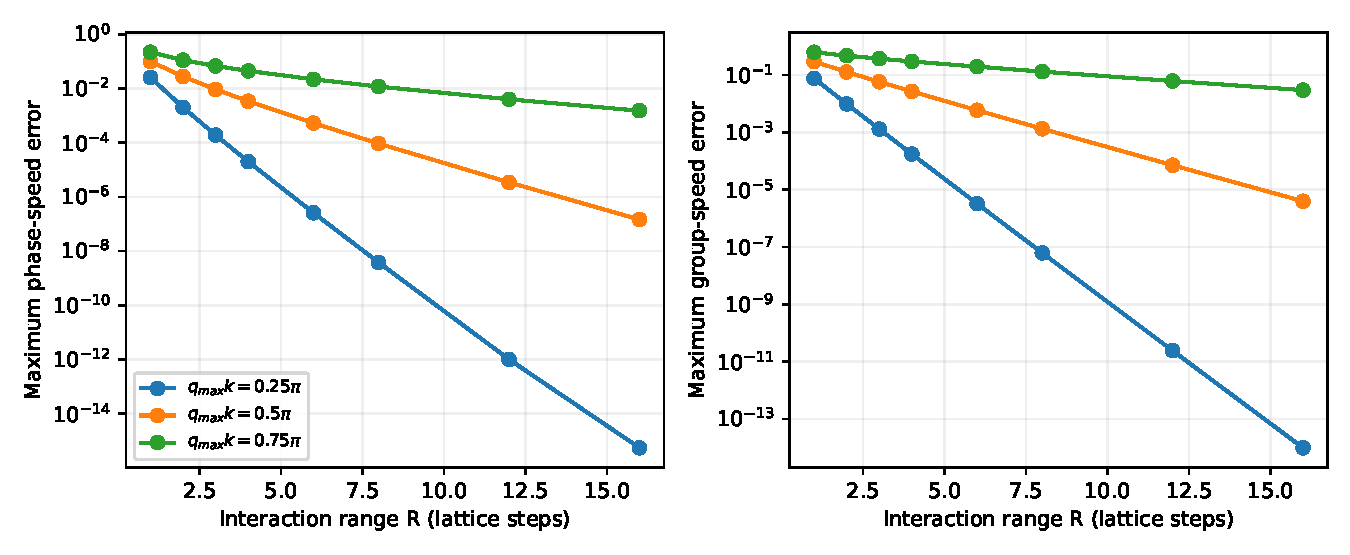
\includegraphics[width=.92\linewidth]{figures/convergence.pdf}
\captionof{figure}{Band errors for the stable centered family. Smaller comparison bands converge more rapidly. Values near $10^{-15}$ encounter the double-precision floor; separate 70-digit endpoint checks are retained in the numerical output.}\label{fig:convergence}
\end{minipage}
\end{center}

\section{What remains unavoidable?}
So far the lattice has become harder to see without becoming any finer. Does that mean it can disappear from wave propagation altogether? The answer depends on whether interaction range is fixed, whether we probe the cutoff, and whether arbitrarily distant couplings are allowed.

\paragraph{Fixed finite range cannot be exactly continuum-like.}
A finite-range lattice has a periodic dispersion function; the continuum target $x^2$ is not periodic. If a finite cosine polynomial $D(x)$ equaled $x^2$ on a nonempty open interval, analyticity would extend that identity to all real $x$, contradicting periodicity. At fixed $R$ the approximation space is finite-dimensional and closed, so a fixed nontrivial band's optimal uniform error is strictly positive. Increasing $R$ changes the class and allows that error to tend to zero. Arbitrarily accurate agreement and exact agreement are different claims.

\paragraph{The edge remains different.}
Near wavelength $2k$, the lattice can no longer imitate a continuum packet speed across the whole band. For every finite-range symmetric rule, $D'(\pi)=0$. If $D(\pi)>0$, then $v_g(\pi)=0$. Consequently its worst group-speed error on the entire closed zone is at least one, regardless of the accuracy at lower wave numbers. This statement excludes rules with a zero-frequency edge, where the square-root derivative needs separate treatment. The centered construction has no such extra zero. Phase speeds can converge even at the edge; group speeds cannot converge uniformly there. This is why the earlier convergence claim stops strictly below the cutoff.

\paragraph{Removing locality changes the answer again.}
Finally, the finite-range restriction itself matters. The absolutely summable infinite-range coefficients
\begin{equation}
 a_r=\frac{2(-1)^{r+1}}{r^2},\qquad r=1,2,\ldots,
\end{equation}
give
\begin{equation}
 2\sum_{r=1}^{\infty}a_r(1-\cos rx)=x^2,
 \qquad -\pi\leq x\leq\pi,
\end{equation}
by the Fourier series of the periodic extension of $x^2$. Thus a stable nonlocal lattice can have exactly continuum dispersion throughout the zone interior. The price is a coupling to arbitrarily distant sites and a derivative mismatch at the identified endpoints of its periodic symbol. Also, the differentiated second-moment series is not absolutely convergent, so the finite-range moment argument cannot simply be applied term by term. Spectral differentiation provides related constructions \cite{trefethen}. This example changes the interaction assumption again; it does not remove the lattice's cutoff or add the continuum's missing wave numbers.

\section{What would a detection have to tell us?}
We began with a proposed route from minimum distance to measurement: a spatial gap changes waves, and a long journey might magnify the change enough to detect. The calculation locates the extra assumption in that route. Positive pair interactions force the earlier quadratic slowdown. A gap and stability alone do not.

Within positive pair interactions, nearest neighbors give the best phase accuracy and the smallest leading slowdown coefficient. Stable signed interactions can instead meet any prescribed finite accuracy on a fixed band below the cutoff as range increases. At fixed finite range a discrepancy remains, and at the cutoff the group-speed difference is unavoidable for the nonzero-frequency edge considered here. Which of these facts becomes experimentally useful depends on independent restrictions on the interactions and on the accessible wavelengths.

For photon timing, the distinction is concrete. Under the additional photon interpretation, Eq.~\eqref{grouporder} moves the first energy-dependent delay to progressively higher orders. A search designed for a quadratic lag can therefore miss the leading signature of these signed models, even before sensitivity becomes the issue. The published quadratic limits continue to constrain the original positive-coupling class in its low-energy regime; they do not become universal bounds on the spacing of every stable lattice model. Conversely, a detected dispersion law would need further interpretation before it identified a microscopic geometry.

The geometric consequences of minimum distance remain intact: changing the couplings has not restored a forbidden triangle or an endlessly bisectable segment. What changes is how geometry becomes visible through a physical process. The next step is to justify an interaction class from additional physics, derive its observable consequences, and then ask which experiment can reach them. These calculations supply that distinction, rather than a new electromagnetic theory or evidence for physical discreteness.

\clearpage
\appendix
\section{A group-speed bound for the centered family}\label{app:speed}
Let $P=P_R$ in Eq.~\eqref{poly}. Since $y'=\sqrt{y(1-y)}$ on $0<x<\pi$,
\begin{equation}
 \left(\frac{v_g}{c}\right)^2=\frac{y(1-y)P'(y)^2}{4P(y)}.
\end{equation}
It suffices to show $G=4P-y(1-y)P'^2\geq0$. Write $P'=\sum_{j=0}^{R-1}d_jy^j$. The coefficients are positive and decrease: $d_0=4$ and $d_j/d_{j-1}=2j/(2j+1)<1$. If $P'^2=\sum_n h_ny^n$, its finite convolution coefficients decrease for $n\geq R-1$: advancing $n$ drops one positive term and decreases each surviving term.

For the full arcsine series, the corresponding expression $G$ vanishes identically. Truncating $P$ after degree $R$ changes $G$ only at order $y^{R+1}$, so all lower coefficients vanish. For $j\geq R+1$ the coefficient of $y^j$ in $G$ is $h_{j-2}-h_{j-1}\geq0$, taking coefficients outside the finite support to be zero. Hence $G\geq0$ on $[0,1]$. Since $P'>0$, the group speed is nonnegative, proving the bound. The script independently checks this polynomial certificate exactly for each tested range.

\section{Computational checks and limitations}
The script checks normalization and canceled moments using rational arithmetic, and verifies the equality between the signed cosine symbol and the positive polynomial using symbolic algebra. This certifies global stability of the centered family and its group-speed bound at the tested ranges. Optimized models have a global coefficient-sign stability certificate, not merely a sampled stability test. Numerical consistency checks compare normalization and the analytical optimum in the positive-coupling class.

Errors are evaluated on 100,001 points per comparison band and over the full zone. Optimization uses sampled constraints, extrema refinement, and a feasibility tolerance of $10^{-10}$. Reported very small errors must be interpreted in light of solver and floating-point tolerances. Seventy-digit endpoint calculations document the roundoff floor for centered rules; they are not certified continuous extrema. The saved coefficients, solver scope, error metrics, and exact-check outcomes are in \texttt{results.json}; plots and a CSV are generated by the same run.

\begin{thebibliography}{9}
\small
\bibitem{minimum} J. R. Landers, \emph{Consequences of Minimum Distance in Mathematics and Physics}, accompanying manuscript (2026).
\bibitem{timing} J. R. Landers, \emph{Photon-Timing Tests of a Minimum-Distance Propagation Model}, accompanying companion note (2026).
\bibitem{nist} NIST Digital Library of Mathematical Functions, \S3.4, Differentiation. \url{https://dlmf.nist.gov/3.4}.
\bibitem{fornberg} B. Fornberg, Generation of finite difference formulas on arbitrarily spaced grids, \emph{Mathematics of Computation} \textbf{51} (1988), 699--706. \href{https://doi.org/10.1090/S0025-5718-1988-0935077-0}{doi:10.1090/S0025-5718-1988-0935077-0}.
\bibitem{trefethen} L. N. Trefethen, \emph{Spectral Methods in MATLAB}, SIAM (2000). \href{https://doi.org/10.1137/1.9780898719598}{doi:10.1137/1.9780898719598}.
\end{thebibliography}
\end{document}
